\documentclass[11pt, twoside]{article} 
% Formatting options
\usepackage[a4paper]{geometry}
\geometry{left=25mm, right=25mm, bottom = 30mm}

\usepackage[utf8]{inputenc}

% positioning of images
\usepackage[export]{adjustbox}
\usepackage{wrapfig}
\usepackage{transparent}
% Apa reference style
% use textcite for in-text references and parencite for parental references
% formatting of hyperlinks for URL coded in blue
\usepackage{url}
\usepackage{hyperref}
% break lines in captions
\usepackage{caption}
%insert pdf to appendix
\usepackage{pdfpages}
% title page
\usepackage{fancyhdr}
\usepackage[dvipsnames]{xcolor}
% define color from university template
\definecolor{uos_red}{RGB}{172, 6, 25}
\definecolor{uos_yellow}{RGB}{251, 185, 0}
\definecolor{uos_greay}{RGB}{207, 207, 207}
\definecolor{cssj_purple}{RGB}{79, 8, 123}
\definecolor{cssj_orange}{RGB}{212, 112, 59}

\hypersetup{colorlinks,
    linkcolor={cssj_purple},
    citecolor={cssj_purple},
    urlcolor={cssj_purple!80!black}
}
% colour package for in-text colour use
\usepackage{eso-pic, graphicx}
% references
\usepackage[natbib=true,backend=biber,sorting=nyt,style=apa,dateabbrev=false]{biblatex}
\renewcommand*{\bibfont}{\fontsize{10}{12}\selectfont}
% add your references to this file
\addbibresource{references.bib}

% colored box packages
\usepackage{tikz,lipsum,lmodern}
\usepackage[most]{tcolorbox}

% hexagonal items
\usepackage{stix2,scalerel,lmodern}
\newcommand \hex{\small\scaleto{\varhexagonblack}{1.4\LMex}}

%------------------HEADER---------------------%
\pagestyle{fancyplain}
\fancyhf{}
\fancyhead[L]{{Cognitive Science Student Journal}}
\fancyhead[R]{\transparent{0.7}Style guide} 
\let\oldheadrule\headrule% Copy \headrule into \oldheadrule
\renewcommand{\headrule}{\color{cssj_purple}\oldheadrule}% Add colour to \headrule
\renewcommand{\headrulewidth}{0.5pt}
\fancyfoot[C]{\thepage}
\renewcommand*\familydefault{\sfdefault} 
%------------------HEADER---------------------%

\begin{document}

\begin{titlepage}

\begin{minipage}{0.3\textwidth}
\includegraphics[width=1\textwidth]{images/CSSJ_logo.png}
\end{minipage} 
\hspace{0.02\linewidth}
\begin{minipage}{0.7\textwidth}
\LARGE\textbf{Cognitive Science Student Journal}

\LARGE{Osnabrück University}
\end{minipage}

\vspace{1cm}
\Huge\textbf{Submission template}

\vspace{1cm}
\begin{tcolorbox}[colback=cssj_purple!80!black ,colframe=cssj_purple!80!black]
\color{white}
\noindent \huge\textbf{Great that you submit your scientific paper!}

\vspace{0.6cm}
\noindent Make sure that you adhere to our \textbf{style guide} and fill out our \textbf{author form}.

\vspace{2cm}
\noindent The submission of your scientific paper is divided into three parts within one LaTeX project, for which we provide individual .tex files:
 \begin{enumerate}
    \item Compact Intro
    \item Information
    \item Text body
  \end{enumerate}
\end{tcolorbox}


\end{titlepage}

\newpage
\section*{How to use}
The Cognitive Science Student Journal Style guide might be studied best as a LaTeX project to understand how commands and styles should be applied.
We recommend to copy out examples to apply in your submission.

\section{Text structure}
To structure your text, use sections and subsections. For each section, subsections should only be used, if there are more than one subsection.

Leave a blank line to start a new paragraph. Do not make use of double blackslashes to force a line break.

\section{Style rules}
\begin{itemize}
    \item[\hex] Use the Cognitive Science Student Journal submission template
    \item[\hex] Capitalisation: The first word of each header is capitalized. In text, capitalization should only be used for names, such as personal names, research areas, specific testing procedures, references to specific figures and tables etc. 
    \item[\hex] Abbreviations might only be used at a bare minimum when long words repeatedly occur, particularly in longer texts. 
    \item[\hex] No bold, no italic
    \item[\hex] Use the following quotation marks: ``quote"
    \item[\hex] Choose either American or British English, or German and be consistent.
    \item[\hex] Academic ``we": If you make use of it, use ``I" for a paper by a single author. E.g. As I have demonstrated in Section 2, ... .
\end{itemize}


\section{Referencing}
\begin{itemize}
    \item[\hex] Reference style: APA 7th Edition for all references including captions of Figures. 
    \item[\hex] Bibtex: use bibtex formats exactly as listed in the provided reference template file as it integrates the APA (7th Edition) referencing style into the bibtex format. Bibtex exportation functions on websites usually do not output the format needed here. Find the respective file within the submission template project.
    \item[\hex] In-text referencing: use \textbackslash textcite\{\} for narrative citation, e.g. \textcite{Zolotarov2022} investigate the octopus' brain. Use \textbackslash parencite\{\} for parenthetical citation, e.g. The octopus has a brain that can be investigated \parencite{Zolotarov2022}. 
\end{itemize}


\section{Figures and tables}
Examples on how to insert figures and tables are given subsequently. A figure or table should have a reference in the text pointing towards it.
As shown with Figure \ref{fig:example_image}, the location of figures and tables in the document will be determined by LaTeX, which should not be changed. To refer to a figure or table in the text, use \textbackslash ref followed by the unique label you defined for the figure.
If you have not created a figure or table yourself, you need to state the reference in the caption, e.g. see Figure \ref{fig:example_graph}.
Use Table \ref{tab:journal-introduction} as a template to fit your content.

\begin{figure}
    \centering
    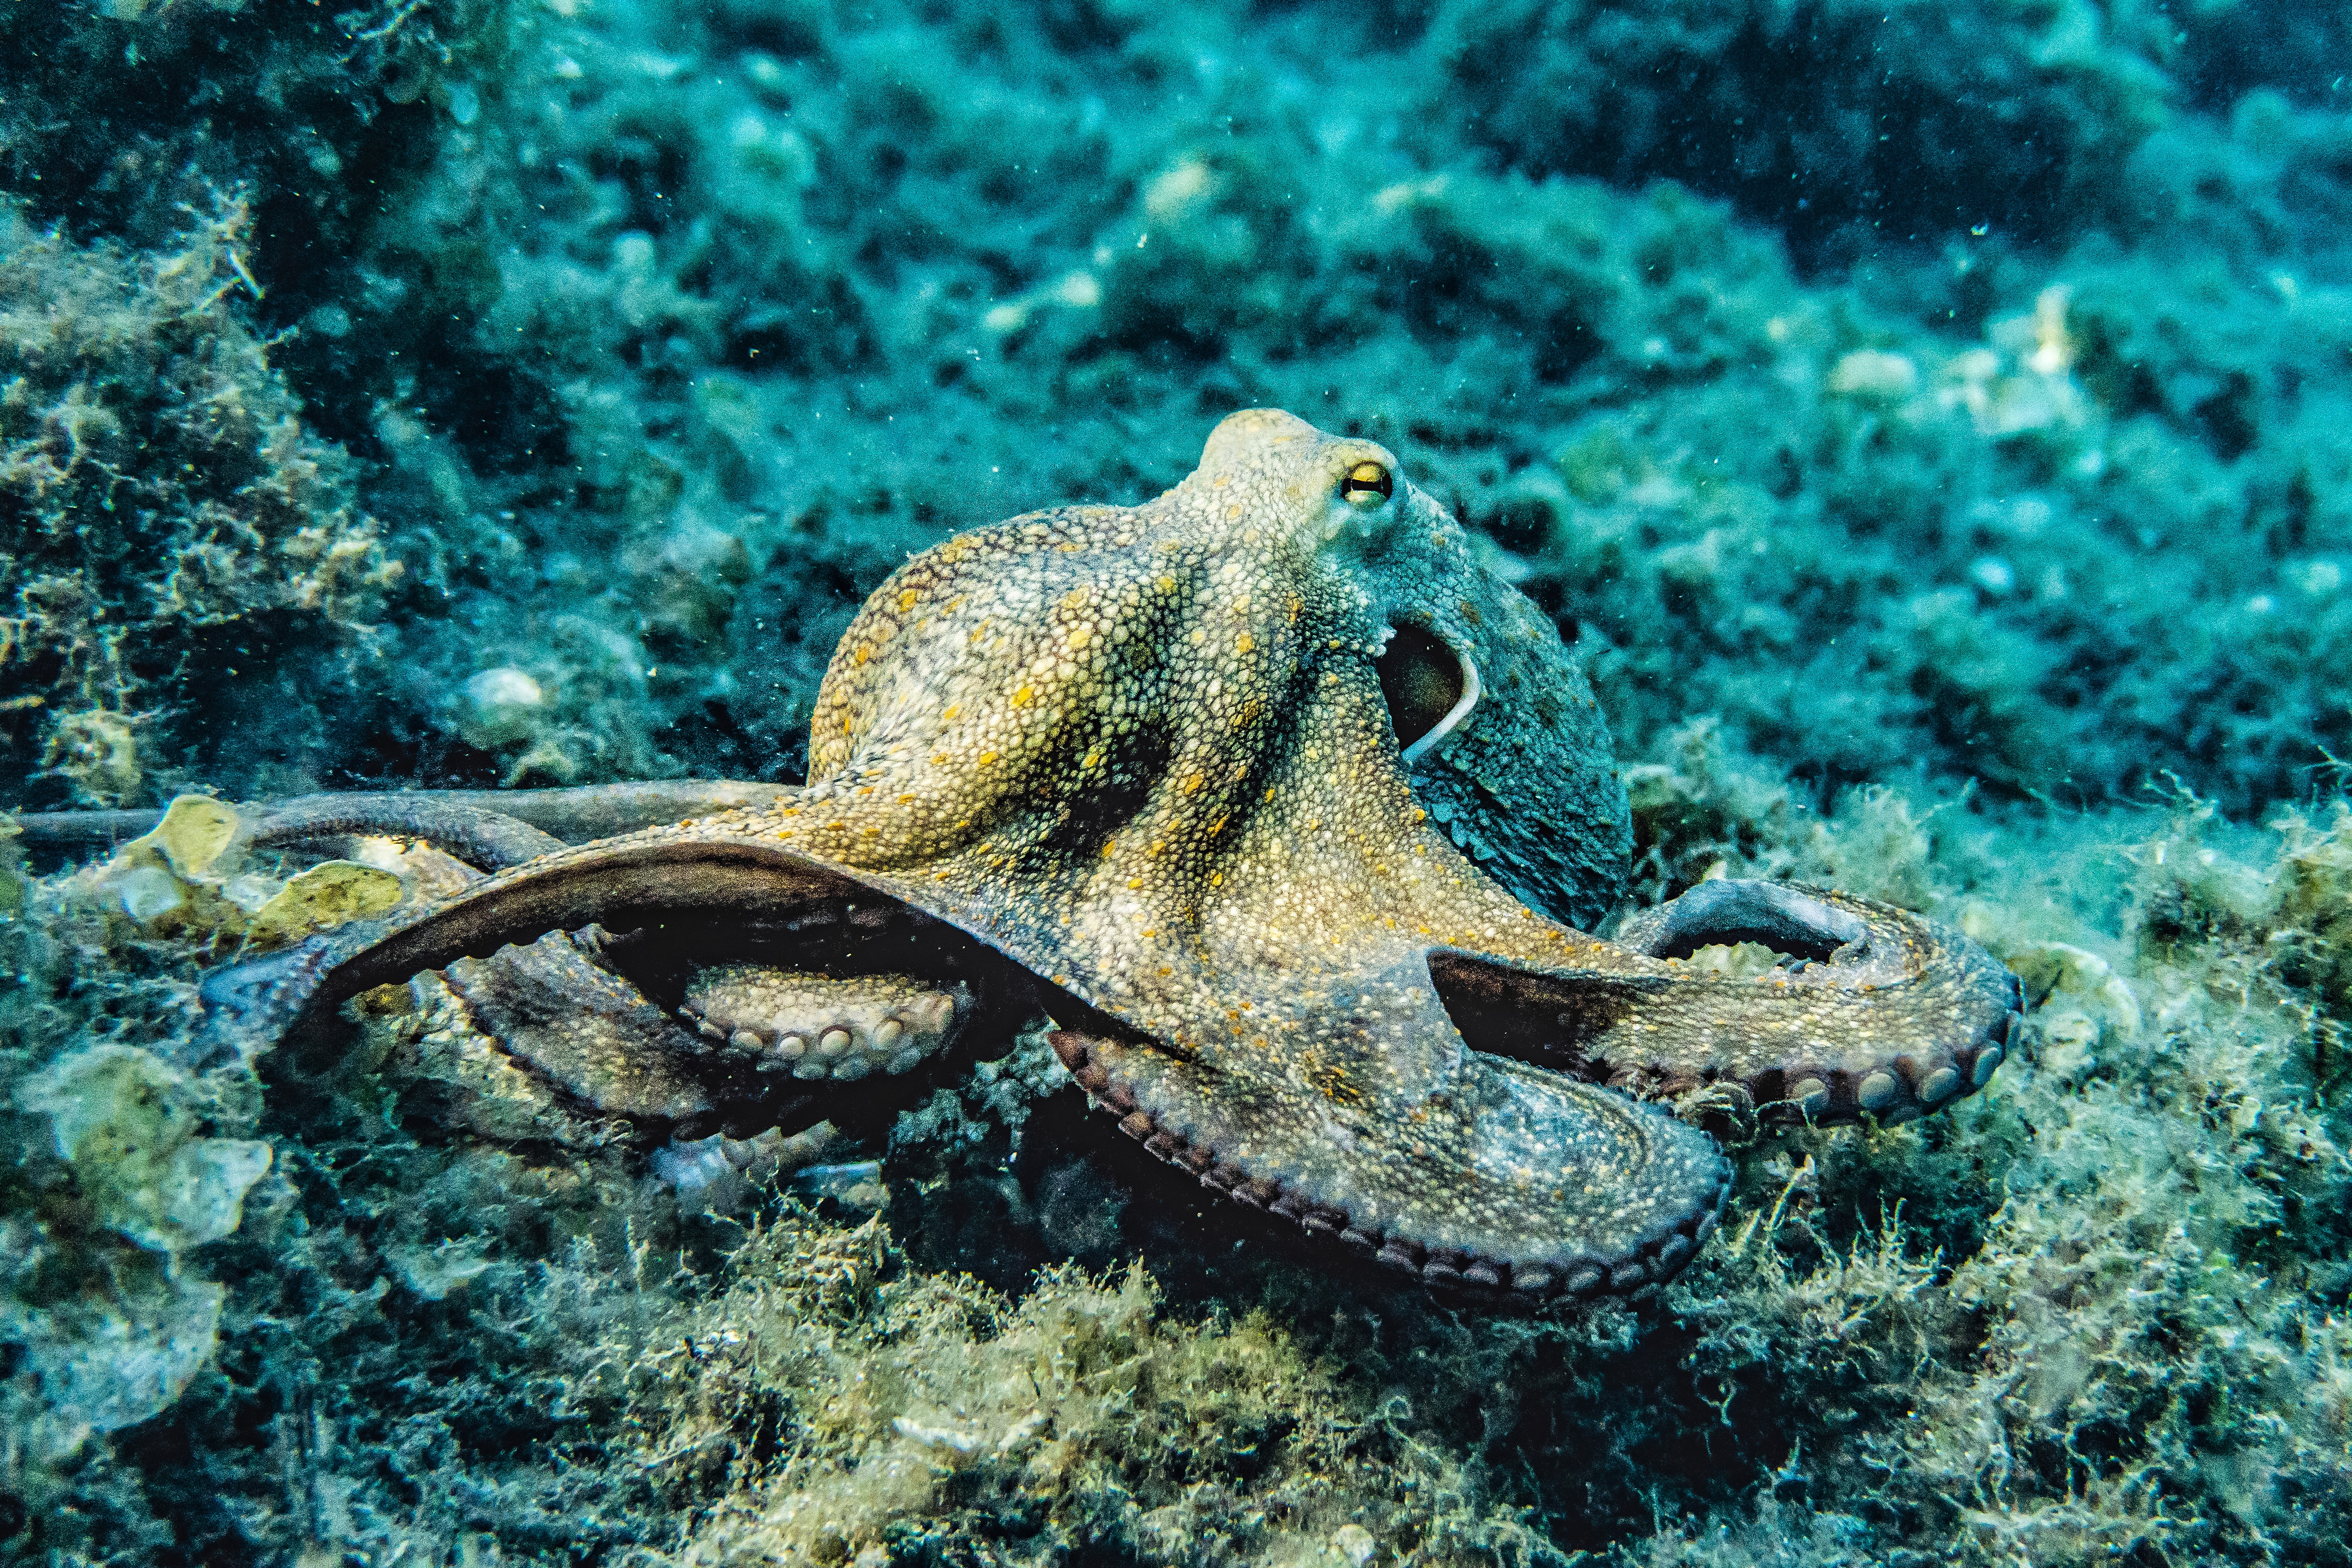
\includegraphics[width=0.4\linewidth]{images/example_image.jpg} % if necessary, change the width of you Figure % change the figures file name respectively
    \caption{Photograph of an Octopus. Adapted from Pia B (https://www.pexels.com/de-de/foto/selektive-fokusfotografie-von-octopus-3046629/)} % adapt the caption 
    \label{fig:example_image} % define a unique label to refer to your Figure
\end{figure}

\begin{figure}
    \centering
    \includegraphics[width=0.8\linewidth]{images/example_image_2.png}
    \caption{RNA profiling of the common octopus O. vulgaris. (A) Schematic representation of tissues sampled in the study. Neuronal and non-neuronal tissues are colored in blue and yellow, respectively. Inset (B): Brain and surrounding structures. (C) Main sequencing methods and computational analyses used in this study. Adapted from \textcite{Zolotarov2022}.}
    \label{fig:example_graph}
\end{figure}

\begin{table}
    \centering
    \begin{tabular}{p{0.3\textwidth}p{0.3\textwidth}p{0.3\textwidth}}
    \hline
    %headline
      Favorite topics & Favorite colors & Favorite social media\\
    \hline
      Cognitive Science & Purple & Instagram\\
      Octopuses & Orange & LinkedIn\\
    \hline
    \end{tabular}
    \caption{The Cognitive Science Student Journal's Favorites} 
    \label{tab:journal-introduction}
\end{table}





\newpage

\printbibliography[]{}
\end{document}
